\chapter{المرشّحات ودوال النقل}\label{ch:b1:filters-transfer-functions}

داخل صندوق مكبّر صوت تقرّر وشيعة ومكثف، دون أيّ
ترانزستور، أن الجهير يذهب إلى المخروط الكبير والحادّ إلى
القبّة الصغيرة. وزرّ ``AC'' في راسم الاهتزاز يزيل إزاحةً
تنجرف ببطء ويبقي التموّج فوقها. ومغذٍّ للاستطاعة يحوّل
تيارًا منزليًّا مقوَّمًا نابضًا إلى توتر ثابت بمكثف واحد.
والثلاثة كلها \emph{مرشّحات}: أي دارات خطية تعامل كل تواتر
معاملة مختلفة. ولأن كل إشارة دورية مجموع جيوب، فمعرفة
ما تفعله دارة بكل جيب --- أي دالة نقلها --- هي
معرفة ما تفعله بكل شيء. ويعرّف هذا الفصل دوال
النقل، ويرسم مخططات بودي لدارات الرتبتين الأولى والثانية في
الفصول السابقة، ويستعملها للتنبؤ بكيفية خروج
موجة مربعة من \omterm{def:b1:filters-transfer-functions:H}{مرشّح}.

\section{دالة النقل ومخطط بودي}

\begin{definition}[دالة النقل]\label{def:b1:filters-transfer-functions:H}
\index{دالة النقل}\index{كسب}\index{مرشّح}
\omterm{def:b1:dc-circuits:linear}{الدارة الخطية} ذات توتر دخل $\underline U_e$ وتوتر
خرج $\underline U_s$ (مأخوذ ولا شيء موصول عند الخرج) لها
\emph{دالة النقل}
\[
\underline H(j\omega) = \frac{\underline U_s}{\underline U_e},
\qquad G(\omega) = \abs{\underline H}, \qquad \varphi(\omega) = \arg\underline H,
\]
حيث \emph{الكسب} $G$ (نسبة السعتين) وانزياح الطور $\varphi$
للخرج بالنسبة إلى الدخل. و\emph{المرشّح} دارة كهذه
تُستعمل لتوقفها على التواتر: فجيب سعته $E$ عند
$\omega$ يخرج $G(\omega)E\cos(\omega t + \varphi(\omega))$.
\end{definition}

\begin{definition}[الديسيبل؛ مخطط بودي]\label{def:b1:filters-transfer-functions:bode}
\index{ديسيبل}\index{مخطط بودي}\index{تواتر القطع}\index{نطاق التمرير}
\omterm{def:b1:filters-transfer-functions:H}{الكسب} \emph{بالديسيبل} هو $G_{\mathrm{dB}} = 20\log_{10}G$: فالعامل
$10$ يساوي \qty{20}{dB}، والعامل $2$ يساوي \qty{6}{dB}، والعامل $1/\sqrt2$ يساوي
\qty{-3}{dB}. ويرسم \emph{مخطط بودي} $G_{\mathrm{dB}}$ و
$\varphi$ بدلالة $\log_{10}\omega$ (أو $f$). و\emph{تواتر
القطع} هو التواتر الذي يهبط عنده $G$ إلى $G_{\max}/\sqrt2$ (أي \qty{-3}{dB} عن
الأعظم)؛ و\emph{نطاق التمرير} هو مجال التواترات الواقعة ضمن
\qty{3}{dB} من الأعظم. والعقد عامل $10$ في التواتر، و
الأوكتاف عامل $2$.
\end{definition}

\begin{method}[طبيعة المرشّح بنظرة واحدة]\label{met:b1:filters-transfer-functions:nature}
قبل الحساب، انظر إلى الحدود: فعند التواتر المنخفض جدًّا يكون المكثف
دارة مفتوحة والوشيعة سلكًا؛ وعند التواتر العالي جدًّا يكون
العكس. استبدل بكلٍّ منهما ما يوافقه واقرأ هل الخرج هو الدخل
(فيمرّر) أم صفر (فيُحجب). فما يمرّر المنخفض ويحجب العالي: تمرير منخفض؛ و
العكس: تمرير عالٍ؛ وما يحجب الاثنين: تمرير نطاقي؛ وما يمرّرهما: إيقاف نطاقي.
ثم احسب $\underline H$ بمجزّئ توتر.
\end{method}

\section{مرشّحات الرتبة الأولى}

\begin{proposition}[تمرير منخفض من الرتبة الأولى]\label{prop:b1:filters-transfer-functions:lowpass1}
\index{مرشّح تمرير منخفض}\index{مكامِل}
مجزّئ RC بخرج على طرفَي $C$ (أو مجزّئ RL بخرج
على طرفَي $R$) له
\[
\underline H = \frac{1}{1 + j\omega/\omega_c}, \qquad
\omega_c = \frac{1}{RC} \ \Big(\text{أو } \frac{R}{L}\Big),
\qquad G = \frac{1}{\sqrt{1 + (\omega/\omega_c)^2}}, \qquad
\varphi = -\arctan\frac{\omega}{\omega_c} .
\]
والمقاربات في \omterm{def:b1:filters-transfer-functions:bode}{مخطط بودي}: $G_{\mathrm{dB}} = 0$ من أجل $\omega \ll \omega_c$، و
مستقيم يهبط \qty{20}{dB} لكل عقد من أجل $\omega \gg \omega_c$،
ويلتقيان عند $\omega_c$ حيث يكون المنحني الحقيقي عند \qty{-3}{dB} و
$\varphi = -45^\circ$. ومن أجل $\omega \gg \omega_c$ يكون $\underline H \approx
\omega_c/(j\omega)$: فيتناسب الخرج مع \emph{تكامل}
الدخل --- أي إن \omterm{def:b1:filters-transfer-functions:H}{المرشّح} مكامِل هناك.
\end{proposition}

\begin{proof}
\omterm{prop:b1:dc-circuits:dividers}{مجزّئ التوتر}:
\[
\underline H = \frac{1/jC\omega}{R + 1/jC\omega} = \frac{1}{1 + jRC\omega} .
\]
وفوق \omterm{def:b1:filters-transfer-functions:bode}{تواتر القطع} بكثير يكون $1 + j\omega/\omega_c \approx j\omega/\omega_c$، و
قسمة \omterm{def:b1:sinusoidal-impedance:complex}{سعة عقدية} على $j\omega$ مكاملةٌ
(\cref{prop:b1:sinusoidal-impedance:rules}): أي $u_s \approx \omega_c\int u_e\,\dd t$.
والمقدار $20\log(\omega_c/\omega)$ يفقد \qty{20}{dB} كلما تضاعف $\omega$ عشر مرات.
\end{proof}

\begin{proposition}[تمرير عالٍ من الرتبة الأولى]\label{prop:b1:filters-transfer-functions:highpass1}
\index{مرشّح تمرير عالٍ}\index{دارة مشتقّة}
مجزّئ CR بخرج على طرفَي $R$ (أو LR بخرج على طرفَي $L$)
له
\[
\underline H = \frac{j\omega/\omega_c}{1 + j\omega/\omega_c},
\qquad G = \frac{\omega/\omega_c}{\sqrt{1 + (\omega/\omega_c)^2}},
\qquad \varphi = \frac{\pi}{2} - \arctan\frac{\omega}{\omega_c},
\]
وهو يرتفع \qty{20}{dB} لكل عقد دون $\omega_c$، ومسطّح فوقه، و\qty{-3}{dB}
و$+45^\circ$ عند $\omega_c$. ومن أجل $\omega \ll \omega_c$ يكون $\underline H
\approx j\omega/\omega_c$: فيتناسب الخرج مع
\emph{مشتقّ} الدخل.
\end{proposition}

\begin{proof}
$\underline H = R/(R + 1/jC\omega) = jRC\omega/(1 + jRC\omega)$؛ و
الضرب في $j\omega$ اشتقاقٌ.
\end{proof}

\begin{omfigure}
\begin{tikzpicture}
\begin{axis}[omaxis, axis x line=bottom, axis y line=left, xlabel style={at={(axis description cs:0.5,-0.14)}, anchor=north}, width=7.4cm, height=5.2cm, xmode=log, xlabel={$\omega/\omega_c$},
    ylabel={$G_{\mathrm{dB}}$}, xmin=0.01, xmax=100, ymin=-42, ymax=6,
    ytick={0,-20,-40}, yticklabels={$0$,$-20$,$-40$},
    xtick={0.01,0.1,1,10,100}, xticklabels={$10^{-2}$,$10^{-1}$,$1$,$10$,$10^{2}$}]
  \addplot[omExo, dashed, domain=0.01:1, samples=2] {0};
  \addplot[omExo, dotted, domain=0.01:100, samples=2] {-3};
  \addplot[omExo, dashed, domain=1:100, samples=2] {-20*log10(x)};
  \addplot[omDef, thick, domain=0.01:100, samples=200] {-10*log10(1 + x^2)};
  \addplot[omThm, thick, domain=0.01:100, samples=200] {-10*log10(1 + 1/x^2)};
  \node[omDef, font=\footnotesize] at (axis cs:0.05,-7) {تمرير منخفض};
  \node[omThm, font=\footnotesize] at (axis cs:30,-9) {تمرير عالٍ};
\end{axis}
\end{tikzpicture}\qquad
\begin{tikzpicture}
\begin{axis}[omaxis, axis x line=bottom, axis y line=left, xlabel style={at={(axis description cs:0.5,-0.14)}, anchor=north}, width=7.0cm, height=5.2cm, xmode=log, xlabel={$\omega/\omega_c$},
    ylabel={$\varphi$}, xmin=0.01, xmax=100, ymin=-1.8, ymax=1.8,
    ytick={-1.5708,-0.7854,0,0.7854,1.5708}, yticklabels={$-\frac{\pi}{2}$,$-\frac{\pi}{4}$,$0$,$\frac{\pi}{4}$,$\frac{\pi}{2}$},
    xtick={0.01,0.1,1,10,100}, xticklabels={$10^{-2}$,$10^{-1}$,$1$,$10$,$10^{2}$}]
  \addplot[omDef, thick, domain=0.01:100, samples=200] {-rad(atan(x))};
  \addplot[omThm, thick, domain=0.01:100, samples=200] {rad(90 - atan(x))};
\end{axis}
\end{tikzpicture}

{\small مخططا بودي للتمرير المنخفض (الأزرق) والتمرير العالي
(الأحمر) من الرتبة الأولى: \omterm{def:b1:filters-transfer-functions:H}{الكسب} \omterm{def:b1:filters-transfer-functions:bode}{بالديسيبل} مع المقاربين (المتقطعين) يلتقيان عند
\omterm{def:b1:filters-transfer-functions:bode}{تواتر القطع}، حيث يكون \omterm{def:b1:filters-transfer-functions:H}{الكسب} الحقيقي \qty{-3}{dB}، ثم الطور، وهو يعبر
$\mp45^\circ$ عند \omterm{def:b1:filters-transfer-functions:bode}{تواتر القطع}.}
\end{omfigure}

\begin{example}[الاقتران المتناوب]\label{ex:b1:filters-transfer-functions:accoupling}
دخل ``AC'' في راسم الاهتزاز \omterm{prop:b1:filters-transfer-functions:highpass1}{مرشّح تمرير عالٍ} عند $f_c \approx \qty{10}{Hz}$:
فإشارة عند \qty{1}{kHz} راكبة على إزاحة قدرها \qty{5}{V} تعبر عند
\qty{-0.0002}{dB} وقد أُزيلت إزاحتها. أما موجة مربعة عند \qty{50}{Hz}
فتتشوّه تشوّهًا مرئيًّا --- إذ تتهدّل قممها المسطّحة --- لأن \omterm{def:b1:filters-transfer-functions:H}{المرشّح} عند
\qty{50}{Hz} لا يعلو تواترَ قطعه إلا بعقد واحد ولأن توافقيات الإشارة
المنخفضة تنزاح في الطور
(\cref{exo:b1:filters-transfer-functions:12}).
\end{example}

\section{مرشّحات الرتبة الثانية}

\begin{proposition}[الدارة RLC على التسلسل ثلاثةَ مرشّحات]\label{prop:b1:filters-transfer-functions:rlc}
\index{مرشّح تمرير نطاقي}\index{مرشّح من الرتبة الثانية}
مع $x = \omega/\omega_0$ و $\omega_0 = 1/\sqrt{LC}$ و $Q =
\sqrt{L/C}/R$، تعطي \omterm{prop:b1:transient-regimes:rlc}{الدارة RLC} على التسلسل المغذّاة بالتوتر $\underline U_e$، حسب
موضع أخذ الخرج:
\begin{align*}
\text{على طرفَي } C:&\quad \underline H = \frac{1}{1 - x^2 + jx/Q}, \\
\text{على طرفَي } R:&\quad \underline H = \frac{jx/Q}{1 - x^2 + jx/Q} = \frac{1}{1 + jQ(x - 1/x)}, \\
\text{على طرفَي } L:&\quad \underline H = \frac{-x^2}{1 - x^2 + jx/Q}:
\end{align*}
أي \omterm{prop:b1:filters-transfer-functions:lowpass1}{مرشّح تمرير منخفض} وآخر تمرير نطاقي وثالث تمرير عالٍ من الرتبة الثانية. وبعيدًا عن
$\omega_0$ يهبط التمرير المنخفض والتمرير العالي \qty{40}{dB} لكل عقد، و
يهبط التمرير النطاقي \qty{20}{dB} لكل عقد على كل جانب؛ ويبلغ التمرير النطاقي
أعظمه $1$ عند $\omega_0$ وله \omterm{thm:b1:sinusoidal-impedance:resonance}{عرض النطاق} $\Delta\omega =
\omega_0/Q$ في \cref{thm:b1:sinusoidal-impedance:resonance}.
\end{proposition}

\begin{proof}
مجزّئات توتر \omterm{def:b1:sinusoidal-impedance:impedance}{بالممانعة} الكلية $R + j(L\omega - 1/C\omega)$؛
ثم نضرب البسط والمقام في $jC\omega$ ونستعمل
$LC\omega_0^2 = 1$ و $RC\omega_0 = 1/Q$. والتمرير النطاقي هو رنين
التيار في الفصل السابق مقروءًا توترًا على طرفَي $R$.
\end{proof}

\begin{proposition}[تمرير منخفض من الرتبة الثانية: دور $Q$]\label{prop:b1:filters-transfer-functions:lowpass2}
\index{رنين!مرشّح}
من أجل التمرير المنخفض، $G = 1/\sqrt{(1 - x^2)^2 + x^2/Q^2}$: فمن أجل
$Q > 1/\sqrt2$ يرتفع \omterm{def:b1:filters-transfer-functions:H}{الكسب} فوق $1$ قرب $\omega_0$ (أي رنين، وذروته
$\approx Q$ من أجل $Q$ كبير)؛ ومن أجل $Q = 1/\sqrt2$ يكون ``مسطّحًا إلى أقصى حدّ''،
$G = 1/\sqrt{1 + x^4}$، وعند \qty{-3}{dB} بالضبط عند $\omega_0$؛ ومن أجل $Q$ أصغر
يتهدّل مبكرًا. ويسير الطور من $0$ إلى $-\pi$، مارًّا بالقيمة $-\pi/2$
عند $\omega_0$.
\end{proposition}

\begin{proof}
$(1 - x^2)^2 + x^2/Q^2 = 1 + x^4 + x^2(1/Q^2 - 2)$: فالحدّ الأوسط
ينعدم من أجل $Q^2 = \tfrac12$، ويكون سالبًا (فذروة) فوقه، وموجبًا
(فتهدّل) دونه؛ وقد حُلّل السلوك قرب $x = 1$ في
\cref{prop:b1:sinusoidal-impedance:overvoltage}.
\end{proof}

\begin{omfigure}
\begin{tikzpicture}
\begin{axis}[omaxis, axis x line=bottom, axis y line=left, xlabel style={at={(axis description cs:0.5,-0.14)}, anchor=north}, width=7.4cm, height=5.4cm, xmode=log, xlabel={$\omega/\omega_0$},
    ylabel={$G_{\mathrm{dB}}$}, xmin=0.1, xmax=10, ymin=-45, ymax=15,
    ytick={10,0,-20,-40}, xtick={0.1,1,10}, xticklabels={$0.1$,$1$,$10$},
    legend style={at={(0.03,0.03)}, anchor=south west, font=\footnotesize, draw=none, fill=none}]
  \addplot[omDef, thick, domain=0.1:10, samples=300] {-10*log10((1 - x^2)^2 + x^2/9)};
  \addlegendentry{$Q = 3$}
  \addplot[omThm, thick, domain=0.1:10, samples=300] {-10*log10(1 + x^4)};
  \addlegendentry{$Q = 1/\sqrt2$}
  \addplot[omProp, thick, domain=0.1:10, samples=300] {-10*log10((1 - x^2)^2 + x^2/0.04)};
  \addlegendentry{$Q = 0.2$}
  \addplot[omExo, dashed, domain=1:10, samples=2] {-40*log10(x)};
\end{axis}
\end{tikzpicture}\qquad
\begin{tikzpicture}
\begin{axis}[omaxis, axis x line=bottom, axis y line=left, xlabel style={at={(axis description cs:0.5,-0.14)}, anchor=north}, width=7.0cm, height=5.4cm, xmode=log, xlabel={$\omega/\omega_0$},
    ylabel={$G_{\mathrm{dB}}$}, xmin=0.1, xmax=10, ymin=-45, ymax=5,
    ytick={0,-20,-40}, xtick={0.1,1,10}, xticklabels={$0.1$,$1$,$10$},
    legend style={at={(0.03,0.97)}, anchor=north west, font=\footnotesize, draw=none, fill=none}]
  \addplot[omExo, dotted, domain=0.1:10, samples=2, forget plot] {-3};
  \addplot[omDef, thick, domain=0.1:10, samples=400] {-10*log10(1 + 100*(x - 1/x)^2)};
  \addlegendentry{$Q = 10$}
  \addplot[omThm, thick, domain=0.1:10, samples=300] {-10*log10(1 + (x - 1/x)^2)};
  \addlegendentry{$Q = 1$}
\end{axis}
\end{tikzpicture}

{\small مرشّحات من الرتبة الثانية من \omterm{prop:b1:transient-regimes:rlc}{الدارة RLC} على التسلسل. يسارًا: التمرير المنخفض
(الخرج على طرفَي $C$) من أجل ثلاث قيم \omterm{def:b1:transient-regimes:secondorder}{لعامل الجودة} $Q$: ذروة رنين، أو استجابة
مسطّحة إلى أقصى حدّ، أو تهدّل مبكر، وكلها تلتحق بالمقارب
\qty{-40}{dB/decade} (المتقطع). ويمينًا: التمرير النطاقي (الخرج على طرفَي $R$): ذروة
عرضها $\omega_0/Q$ تهبط \qty{20}{dB/decade} على كل جانب.}
\end{omfigure}

\begin{example}[شبكة فصل]\label{ex:b1:filters-transfer-functions:crossover}
مجهار الجهير ومجهار الحدّة في مكبّر صوت، وكلاهما \qty{8}{\ohm}، يتقاسمان
المضخّم عبر \omterm{prop:b1:filters-transfer-functions:lowpass1}{مرشّح تمرير منخفض} (وشيعة على التسلسل) \omterm{prop:b1:filters-transfer-functions:highpass1}{ومرشّح تمرير عالٍ} (مكثف على
التسلسل) بتواتر فصل \qty{2}{kHz}: أي $L = R/\omega_c = \qty{0.64}{mH}$ و
$C = 1/R\omega_c = \qty{10}{\micro F}$. وعند \qty{2}{kHz} يأخذ كل مجهار
\qty{-3}{dB}، أي نصف الاستطاعة، ويكون $G_L^2 + G_H^2 = 1$ عند كل
تواتر: فالاستطاعة مقتسَمة لا ضائعة. وتصمّم مسألة نهاية الأسبوع
نسخة أشدّ انحدارًا.
\end{example}

\section{ترشيح إشارة دورية}

\begin{theorem}[تفكيك فورييه]\label{thm:b1:filters-transfer-functions:fourier}
\index{متسلسلة فورييه}\index{توافقي}\index{طيف!إشارة دورية}
كل إشارة دورية دورها $T = 2\pi/\omega$ (منتظمة بما فيه الكفاية) هي
مجموع ثابت وجيوب عند مضاعفات $\omega$:
\[
s(t) = c_0 + \sum_{n = 1}^{\infty} c_n\cos(n\omega t + \varphi_n),
\]
حيث $c_0 = \langle s\rangle$ قيمتها المتوسطة؛ والحدّ $n = 1$ هو
\emph{الأساسي}، والباقي \emph{التوافقيات}، وتشكّل
السعات $c_n$ \emph{الطيف}. وللموجة المربعة ذات السعة
$\pm E$ يكون $c_n = 4E/(n\pi)$ من أجل $n$ فردي و $0$ من أجل $n$ زوجي؛ وللموجة
المثلثية ذات السعة $\pm E$ يكون $c_n = 8E/(n\pi)^2$ من أجل $n$ فردي.
\end{theorem}
\admitted

\begin{remark}[ما يُؤخذ منها]\label{rem:b1:filters-transfer-functions:fourier}
المبرهنة وحساب المعاملات $c_n$ ينتميان إلى درس رياضيات السنة
الثانية. وهي هنا أداة: فالزوايا الحادّة تحتاج إلى توافقيات كثيرة
(إذ تتناقص توافقيات الموجة المربعة بالمقدار $1/n$ فقط)، والإشارات السلسة
تحتاج إلى قليل منها (وتتناقص توافقيات المثلثية بالمقدار $1/n^2$). والمحتوى التوافقي للإشارة
هو ما يتكوّن منه جرس الآلة، وما يعمل عليه \omterm{def:b1:filters-transfer-functions:H}{المرشّح}.
\end{remark}

\begin{proposition}[الترشيح الخطي لإشارة دورية]\label{prop:b1:filters-transfer-functions:filtering}
عبر \omterm{def:b1:filters-transfer-functions:H}{مرشّح} دالة نقله $\underline H$، تصير إشارة
المبرهنة
\[
s_{\text{خرج}}(t) = G(0)\,c_0 + \sum_{n \geq 1} G(n\omega)\,c_n\cos\!\big(n\omega t + \varphi_n + \varphi(n\omega)\big):
\]
أي إن كل توافقي يُضرب في \omterm{def:b1:filters-transfer-functions:H}{الكسب} ويُزاح بالطور عند
تواتره \emph{هو}، ثم تُجمع القطع. ومن ثمّ:
\begin{itemize}
  \item \omterm{prop:b1:filters-transfer-functions:lowpass1}{مرشّح تمرير منخفض} مع $\omega_c \ll \omega$ يبقي $c_0$ أساسًا:
        فهو \emph{يتوسّط} (أي يملّس ويزيل التموّج)، ويحوّل
        موجة مربعة إلى مثلث صغير (بالمكاملة)؛
  \item \omterm{prop:b1:filters-transfer-functions:highpass1}{مرشّح تمرير عالٍ} مع $\omega_c \ll \omega$ يزيل $c_0$ ويمرّر
        الباقي (وهو الاقتران المتناوب)؛ ومع $\omega_c \gg \omega$
        يشتقّ (فينشئ نتوءات عند حواف الموجة المربعة)؛
  \item \omterm{prop:b1:filters-transfer-functions:rlc}{ومرشّح تمرير نطاقي} مضبوط على $n\omega$ مع $Q \gg 1$ يستخرج
        التوافقي $n$ وحده: أي جيبًا من موجة مربعة.
\end{itemize}
\end{proposition}

\begin{proof}
التراكب في \omterm{def:b1:dc-circuits:linear}{دارة خطية} (\cref{thm:b1:dc-circuits:superposition})
مطبَّقًا على مجموع مداخل جيبية، وكلٌّ منها معالَج وفق
\cref{def:b1:filters-transfer-functions:H}.
\end{proof}

\begin{omfigure}
\begin{tikzpicture}
\begin{axis}[omaxis, axis x line=bottom, width=6.6cm, height=4.8cm, xlabel={التوافقي $n$}, ylabel={$c_n/c_1$},
    xmin=0, xmax=10, ymin=0, ymax=1.15, xtick={1,3,5,7,9}, ytick={0.5,1}]
  \addplot[ybar, bar width=7pt, fill=omDef!35, draw=omDef] coordinates {(1,1) (3,0.333) (5,0.2) (7,0.143) (9,0.111)};
  \addplot[ybar, bar width=3.5pt, fill=omThm, draw=omThm] coordinates
    {(1,0.7071) (3,0.1054) (5,0.0392) (7,0.0202) (9,0.0123)};
  \node[omDef, font=\footnotesize] at (axis cs:6.0,0.9) {موجة مربعة (أزرق)};
  \node[omThm, font=\footnotesize] at (axis cs:6.0,0.7) {بعد تمرير منخفض (أحمر)};
\end{axis}
\end{tikzpicture}\hfill
\begin{tikzpicture}
\begin{axis}[omaxis, axis x line=bottom, width=6.6cm, height=4.8cm, xlabel={$t/T$}, ylabel={$u$},
    xmin=0, xmax=2, ymin=-1.3, ymax=1.3, xtick={0.5,1,1.5,2}, ytick={-1,1}, yticklabels={$-E$,$E$}]
  % square wave
  \addplot[omDef!60, thick, const plot, domain=0:2, samples=5] coordinates {(0,1) (0.5,-1) (1,1) (1.5,-1) (2,-1)};
  % RC response with tau = T/(2pi) (wc = w): on each half period u = s + (u0 - s) e^{-t/tau}; steady amplitude A = tanh(T/(4 tau)) = tanh(pi/2)=0.917
  \addplot[omThm, thick, domain=0:0.5, samples=60] {1 - (1 + 0.917)*exp(-2*pi*x)};
  \addplot[omThm, thick, domain=0.5:1, samples=60] {-1 + (1 + 0.917)*exp(-2*pi*(x-0.5))};
  \addplot[omThm, thick, domain=1:1.5, samples=60] {1 - (1 + 0.917)*exp(-2*pi*(x-1))};
  \addplot[omThm, thick, domain=1.5:2, samples=60] {-1 + (1 + 0.917)*exp(-2*pi*(x-1.5))};
  % tau = T/(20 pi): wc = 10 w: amplitude tanh(5 pi)=1
  \addplot[omProp, thick, domain=0:0.5, samples=80] {1 - 2*exp(-20*pi*x)};
  \addplot[omProp, thick, domain=0.5:1, samples=80] {-1 + 2*exp(-20*pi*(x-0.5))};
  \addplot[omProp, thick, domain=1:1.5, samples=80] {1 - 2*exp(-20*pi*(x-1))};
  \addplot[omProp, thick, domain=1.5:2, samples=80] {-1 + 2*exp(-20*pi*(x-1.5))};
\end{axis}
\end{tikzpicture}

{\small موجة مربعة عبر \omterm{prop:b1:filters-transfer-functions:lowpass1}{مرشّح تمرير منخفض} من الرتبة الأولى. يسارًا:
طيفها (توافقيات فردية بالمقدار $1/n$) والطيف بعد \omterm{def:b1:filters-transfer-functions:H}{مرشّح} مقطوع
عند الأساسي. ويمينًا: الإشارة الزمنية من أجل $\omega_c = \omega$ (الأحمر،
أقواس أسّية) ومن أجل $\omega_c = 10\omega$ (البرتقالي، زوايا مستديرة
فقط)؛ ومع $\omega_c \ll \omega$ يكون الخرج مثلثًا صغيرًا
حول المتوسط.}
\end{omfigure}

\begin{example}[أعداد]\label{ex:b1:filters-transfer-functions:numbers}
موجة مربعة عند \qty{1}{kHz} سعتها \qty{5}{V}: توافقياتها
\qty{6.37}{V} عند \qty{1}{kHz}، و\qty{2.12}{V} عند \qty{3}{kHz}، و
\qty{1.27}{V} عند \qty{5}{kHz}. وعبر \omterm{def:b1:filters-transfer-functions:H}{مرشّح} RC تمرير منخفض مقطوع عند
\qty{10}{Hz} ($\tau = \qty{16}{ms}$) يكون الخرج مثلثًا سعته
$ET/4\tau \approx \qty{80}{mV}$ حول الصفر؛ وعبر
\omterm{prop:b1:filters-transfer-functions:rlc}{مرشّح تمرير نطاقي} مضبوط على \qty{3}{kHz} مع $Q = 20$، يكون جيبًا قدره \qty{2.1}{V}
عند \qty{3}{kHz} مع بضعة بالمئة فقط من الجارين
(\cref{exo:b1:filters-transfer-functions:8}).
\end{example}

\section{تتالي المرشّحات}

\begin{proposition}[التتالي والتحميل]\label{prop:b1:filters-transfer-functions:cascade}
\index{تتالي المرشّحات}\index{تحميل المرشّح}
لمرشّحين على التتالي $\underline H = \underline H_1\underline H_2$
--- فالكسوب تتضارب، والديسيبلات والأطوار تُجمع --- \emph{شريطة ألّا يحمّل الثاني
الأولَ}، أي ألّا يسحب تيارًا يُذكر من
خرجه. وإلا وجبت إعادة كتابة علاقات المجزّئ للشبكة
المركّبة. أما تابع مضخّم عملياتي
(\cref{ch:b1:operational-amplifier}) بين المرحلتين فيجعل قاعدة الجداء
تامة.
\end{proposition}

\begin{proof}
عُرِّفت $\underline H_1$ وخرجها مفتوح؛ فإذا كانت \omterm{def:b1:sinusoidal-impedance:impedance}{ممانعة} دخل
المرحلة التالية أكبر بكثير من \omterm{def:b1:sinusoidal-impedance:impedance}{ممانعة} خرج المرحلة الأولى
(أي مقاومتها التيفنانية)، بقي توتر الخرج على حاله ورأت
المرحلة الثانية $\underline U_{s1}$ بالضبط دخلًا لها.
\end{proof}

\begin{example}[مرحلتا RC]\label{ex:b1:filters-transfer-functions:tworc}
مرشّحا RC تمرير منخفض متماثلان ظهرًا لظهر \emph{لا} يعطيان
$1/(1 + j\omega/\omega_c)^2$: فالمقاومة $R$ في المرحلة الثانية تحمّل الأولى.
والنتيجة الدقيقة هي $\underline H = 1/[1 - (\omega/\omega_c)^2 +
3j\omega/\omega_c]$، أي \qty{-9.5}{dB} عند $\omega_c$ بدلًا من
\qty{-6}{dB} التي تعد بها قاعدة الجداء، وإن كان الاثنان يبلغان الميل نفسه
\qty{-40}{dB/decade} في النهاية.
\end{example}

\section{تمارين}

\begin{exercise}[$\star$]\label{exo:b1:filters-transfer-functions:1}
حوّل إلى \omterm{def:b1:filters-transfer-functions:bode}{ديسيبل}: الكسوب $0.5$ و $10$ و $1/\sqrt2$ و $100$. وحوّل إلى
نسب: \qty{-40}{dB} و \qty{+6}{dB}. ومرشّحان على التتالي (بلا تحميل)
يعطيان \qty{-6}{dB} و\qty{-20}{dB} عند تواتر ما: فما \omterm{def:b1:filters-transfer-functions:H}{الكسب} الكلي؟
\end{exercise}

\begin{exercise}[$\star$]\label{exo:b1:filters-transfer-functions:2}
\omterm{def:b1:filters-transfer-functions:H}{مرشّح} RC تمرير منخفض، $R = \qty{10}{k\ohm}$ و $C = \qty{16}{nF}$: أوجد \omterm{def:b1:filters-transfer-functions:bode}{تواتر القطع}،
\omterm{def:b1:filters-transfer-functions:H}{والكسب} \omterm{def:b1:filters-transfer-functions:bode}{بالديسيبل} عند \qty{100}{Hz} و\qty{1}{kHz} و\qty{10}{kHz} و
\qty{100}{kHz}.
\end{exercise}

\begin{exercise}[$\star$]\label{exo:b1:filters-transfer-functions:3}
دون حساب، أعطِ طبيعة \omterm{def:b1:filters-transfer-functions:H}{المرشّح} (تمرير منخفض أو عالٍ أو نطاقي) في: (أ)
$R$ على التسلسل و $C$ على طرفَي الخرج؛ (ب) $C$ على التسلسل و $R$ على طرفَي
الخرج؛ (ج) $L$ على التسلسل و $C$ على طرفَي الخرج؛ (د) $L$ و $C$ على
التسلسل و $R$ على طرفَي الخرج.
\end{exercise}

\begin{exercise}[$\star$]\label{exo:b1:filters-transfer-functions:4}
موجة مربعة عند \qty{1.0}{kHz} سعتها \qty{5.0}{V}: أعطِ
تواترات وسعات توافقياتها الثلاثة الأولى غير المعدومة. ولماذا
لا توافقيات زوجية لها؟
\end{exercise}

\begin{exercise}[$\star\star$]\label{exo:b1:filters-transfer-functions:5}
\omterm{def:b1:filters-transfer-functions:H}{مرشّح} CR تمرير عالٍ مقطوع عند \qty{10}{kHz} يتلقى موجة مثلثية
سعتها \qty{1.0}{V} عند \qty{100}{Hz}. فسّر لماذا يتصرف تصرّف
\omterm{prop:b1:filters-transfer-functions:highpass1}{دارة مشتقّة} وأعطِ شكل الخرج وسعته.
\end{exercise}

\begin{exercise}[$\star\star$]\label{exo:b1:filters-transfer-functions:6}
\omterm{def:b1:filters-transfer-functions:H}{مرشّح} RC تمرير منخفض مقطوع عند \qty{10}{Hz} يتلقى موجة مربعة عند
\qty{1.0}{kHz} سعتها $\pm\qty{1.0}{V}$. بيّن أن الخرج مثلث
واحسب سعته.
\end{exercise}

\begin{exercise}[$\star\star$]\label{exo:b1:filters-transfer-functions:7}
\omterm{def:b1:filters-transfer-functions:H}{مرشّح} RLC تمرير منخفض على التسلسل مع $L = \qty{10}{mH}$ و $C = \qty{100}{nF}$: أعطِ
$f_0$؛ وأوجد $R$ التي تعطي الاستجابة المسطّحة إلى أقصى حدّ؛ وأعطِ \omterm{def:b1:filters-transfer-functions:H}{الكسب}
\omterm{def:b1:filters-transfer-functions:bode}{بالديسيبل} عند $f_0$ وعند $10f_0$.
\end{exercise}

\begin{exercise}[$\star\star$]\label{exo:b1:filters-transfer-functions:8}
\omterm{prop:b1:filters-transfer-functions:rlc}{مرشّح تمرير نطاقي} ($Q = 20$) مضبوط على \qty{3.0}{kHz} يتلقى الموجة المربعة عند
\qty{1}{kHz} في \cref{exo:b1:filters-transfer-functions:4}. احسب
\omterm{def:b1:filters-transfer-functions:H}{الكسب} عند $1$ و $3$ و\qty{5}{kHz}، وسعات خرج هذه
التوافقيات؛ وصف الخرج.
\end{exercise}

\begin{exercise}[$\star\star$]\label{exo:b1:filters-transfer-functions:9}
مرشّحا RC تمرير منخفض متماثلان ($R = \qty{1.0}{k\ohm}$ و $C = \qty{159}{nF}$)
على التتالي. احسب \omterm{def:b1:filters-transfer-functions:H}{دالة النقل} الدقيقة (فالثاني يحمّل
الأول) \omterm{def:b1:filters-transfer-functions:H}{والكسب} عند $\omega_c = 1/RC$؛ وقارنه بجداء
الكسبين المنفصلين.
\end{exercise}

\begin{exercise}[$\star\star\star$]\label{exo:b1:filters-transfer-functions:10}
ارسم مقاربات بودي للدالة $\underline H = (1 + j\omega/\omega_1)/
(1 + j\omega/\omega_2)$ مع $\omega_1 = \qty{100}{rad/s}$ و $\omega_2 =
\qty{1e4}{rad/s}$: الميول والزوايا والمستوى الأفقي عند التواترات العالية
\omterm{def:b1:filters-transfer-functions:bode}{بالديسيبل}، والطور عند $\sqrt{\omega_1\omega_2}$.
\end{exercise}

\begin{exercise}[$\star\star\star$]\label{exo:b1:filters-transfer-functions:11}
جيب مقوَّم تقويمًا كاملًا (تيار منزلي عند \qty{50}{Hz}) متوسطه $2E/\pi$ و
توافقيه الأول عند \qty{100}{Hz} سعته $4E/3\pi$. ويجب على \omterm{def:b1:filters-transfer-functions:H}{مرشّح} RC
تمرير منخفض أن يخفض تموّج \qty{100}{Hz} دون $1\%$ من
المتوسط: أوجد \omterm{def:b1:filters-transfer-functions:bode}{تواتر القطع} اللازم \omterm{def:b1:transient-regimes:firstorder}{وثابت الزمن}. ولماذا يكون
المكثف وحده (مع مقاومة الحمولة) هو الخيار المعتاد؟
\end{exercise}

\begin{exercise}[$\star\star\star$]\label{exo:b1:filters-transfer-functions:12}
الاقتران المتناوب في راسم اهتزاز \omterm{prop:b1:filters-transfer-functions:highpass1}{مرشّح تمرير عالٍ} مع $C = \qty{0.10}{\micro F}$
و $R = \qty{160}{k\ohm}$. احسب $f_c$. ثم تُطبَّق موجة مربعة: بيّن
أن كل قمة مسطّحة تصير أسّيًّا متناقصًا واحسب التهدّل
(أي الكسر الضائع على نصف دور) عند \qty{50}{Hz} وعند \qty{1}{kHz}.
\end{exercise}

\begin{omfigure}
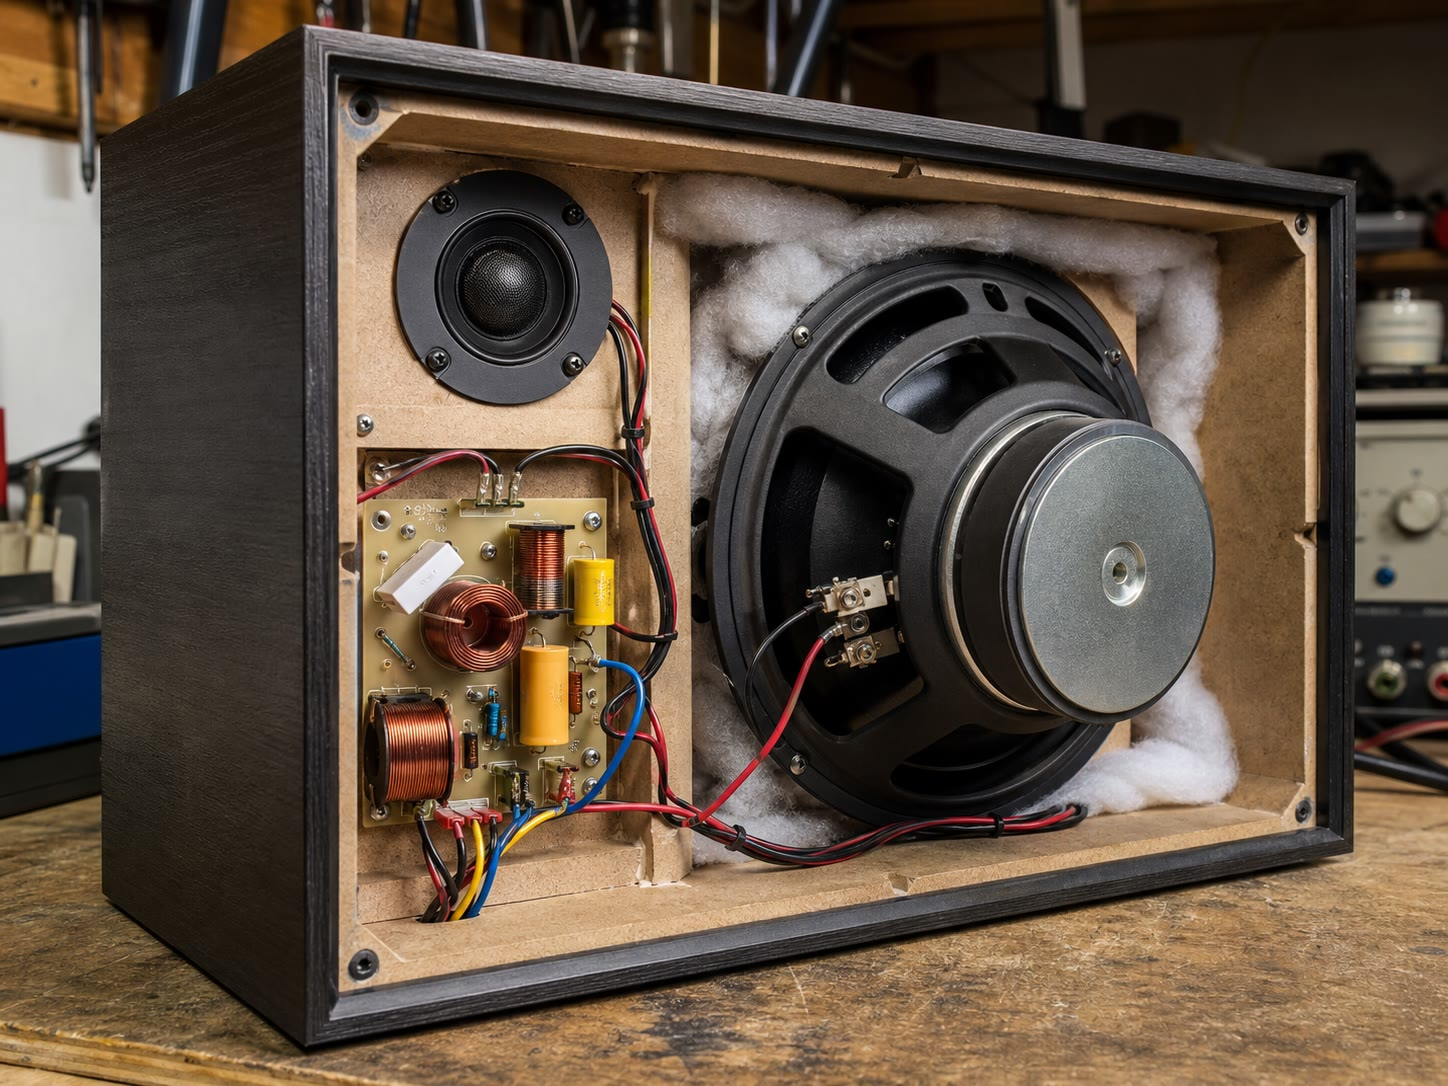
\includegraphics[width=0.50\linewidth]{images/book3/ai/b3-09-loudspeaker-crossover.jpg}

{\small داخل مكبّر صوت ثنائي الطريق: وشائع شبكة الفصل ومكثفاتها هي مرشّحا التمرير المنخفض والتمرير العالي اللذان يرسلان الجهير إلى المجهار الجهيري والحدّة إلى المجهار الحادّ.}
\end{omfigure}

\section{مسألة: شبكة الفصل في مكبّر الصوت}

\begin{problem}[{مسألة نهاية الأسبوع --- مجهار جهيري ومجهار حادّ ووشيعة و
مكثف: كيف تقسم شبكة فصل سلبية الموسيقى، ولماذا تسرّب أبسطها
الجهير إلى المجهار الحادّ، وماذا تفعل وشيعة صوت حقيقية في
التصميم}]
\label{pb:b1:filters-transfer-functions:1}
يُنمذَج المجهار الجهيري والمجهار الحادّ أولًا بمقاومتين خالصتين
$R = \qty{8.0}{\ohm}$. والمضخّم \omterm{def:b1:dc-circuits:sources}{منبع توتر} مثالي
$\underline U_e$. وتواتر الفصل $f_c = \qty{2.0}{kHz}$.

\medskip
\noindent\textbf{الجزء I --- شبكة فصل من الرتبة الأولى.}
يُغذَّى المجهار الجهيري عبر وشيعة $L$ على التسلسل، ويُغذَّى المجهار الحادّ عبر
مكثف $C$ على التسلسل.
\begin{enumerate}
  \item عرّف \omterm{def:b1:filters-transfer-functions:H}{دالة النقل} لكل فرع (التوتر على طرفَي
        المجهار على $\underline U_e$) \omterm{def:b1:filters-transfer-functions:H}{والكسب} \omterm{def:b1:filters-transfer-functions:bode}{بالديسيبل}.
  \item بيّن أن فرع المجهار الجهيري \omterm{prop:b1:filters-transfer-functions:lowpass1}{مرشّح تمرير منخفض} من الرتبة الأولى وأعطِ
        تواتر قطعه $\omega_c$ بدلالة $R$ و $L$.
  \item احسب $L$ من أجل $f_c = \qty{2.0}{kHz}$.
  \item بيّن أن فرع المجهار الحادّ \omterm{prop:b1:filters-transfer-functions:highpass1}{مرشّح تمرير عالٍ} من الرتبة الأولى؛ وأعطِ
        $\omega_c$ واحسب $C$.
  \item أعطِ \omterm{def:b1:filters-transfer-functions:H}{كسب} كل مجهار \omterm{def:b1:filters-transfer-functions:bode}{بالديسيبل} عند $f_c$ وعند \qty{200}{Hz}
        وعند \qty{20}{kHz}.
  \item بيّن أن $G_L^2 + G_H^2 = 1$ عند كل تواتر. وماذا يعني
        ذلك بالنسبة إلى الاستطاعة المسحوبة من المضخّم؟
  \item أعطِ طور كل فرع عند $f_c$؛ وبأيّ مقدار يختلف توترا
        المجهارين في الطور هناك؟
  \item ما ميلا الاستجابتين، \omterm{def:b1:filters-transfer-functions:bode}{بالديسيبل} لكل أوكتاف، بعيدًا
        عن $f_c$؟
\end{enumerate}

\medskip
\noindent\textbf{الجزء II --- شبكة فصل من الرتبة الثانية.}
يُغذَّى المجهار الجهيري الآن عبر وشيعة $L$ على التسلسل مع مكثف $C$
على التفرع مع المجهار.
\begin{enumerate}[resume]
  \item بيّن أن $\underline H = 1/(1 - LC\omega^2 + jL\omega/R)$.
  \item عيّن $\omega_0$ و $Q$ بدلالة $L$ و $C$ و $R$.
  \item من أجل $Q = 1/\sqrt2$ بيّن أن $G = 1/\sqrt{1 + (\omega/\omega_0)^4}$
        وأن \omterm{def:b1:filters-transfer-functions:H}{الكسب} \qty{-3}{dB} عند $\omega_0$.
  \item احسب $L$ و $C$ من أجل $f_0 = \qty{2.0}{kHz}$ و $Q = 1/\sqrt2$.
  \item احسب \omterm{def:b1:filters-transfer-functions:H}{الكسب} \omterm{def:b1:filters-transfer-functions:bode}{بالديسيبل} عند \qty{4}{kHz} و\qty{8}{kHz}؛
        واستنتج الميل \omterm{def:b1:filters-transfer-functions:bode}{بالديسيبل} لكل أوكتاف.
  \item يبادل فرع المجهار الحادّ دورَي $L$ و $C$ ($C$ على التسلسل و
        $L$ على التفرع): اكتب دالة نقله دون حساب
        جديد.
  \item احسب طور كل فرع عند $f_0$. وما الذي يجب فعله في
        توصيل المجهار الحادّ، ولماذا؟
\end{enumerate}

\medskip
\noindent\textbf{الجزء III --- الموسيقى عبر شبكة الفصل.}
\begin{enumerate}[resume]
  \item نغمة تشيلو عند \qty{220}{Hz} تحمل توافقيات حتى التوافقي العشرين.
        فأيّ التوافقيات تذهب في معظمها إلى المجهار الحادّ مع شبكة الفصل
        من الرتبة الأولى؟
  \item وماذا يحدث للتوافقي التاسع؟
  \item تُستعمل موجة مربعة عند \qty{1.0}{kHz} إشارةَ اختبار. ومع
        شبكة الفصل من الرتبة الأولى، أعطِ \omterm{def:b1:filters-transfer-functions:H}{كسب} كل فرع من أجل
        أساسيها وتوافقيها الثالث والخامس.
  \item يطوّر المضخّم بالخطأ إزاحة مستمرة قدرها \qty{1}{V}. فأيّ
        مجهار محمي، وبأيّ شيء؟
  \item مع شبكة الفصل من الرتبة الأولى، أيّ كسر من توتر نغمة عند
        \qty{500}{Hz} ومن استطاعتها يبلغ المجهار الحادّ؟
        والمثل مع الرتبة الثانية. ولماذا يهمّ ذلك
        في بقاء المجهار الحادّ؟
\end{enumerate}

\medskip
\noindent\textbf{الجزء IV --- وشيعة صوت حقيقية.}
المجهار الجهيري هو في الواقع $R = \qty{8.0}{\ohm}$ على التسلسل مع تحريضية
وشيعة صوت $L_{vc} = \qty{0.50}{mH}$.
\begin{enumerate}[resume]
  \item احسب \omterm{def:b1:sinusoidal-impedance:impedance}{ممانعة} المجهار الجهيري (المقياس) عند \qty{2}{kHz} وعند
        \qty{8}{kHz}.
  \item أعد حساب \omterm{def:b1:filters-transfer-functions:H}{كسب} المجهار الجهيري من الرتبة الأولى عند \qty{2}{kHz} و
        \qty{8}{kHz} بهذه \omterm{def:b1:sinusoidal-impedance:impedance}{الممانعة}، وقارنه بالقيمتين المثاليتين
        \qty{-3}{dB} و\qty{-12.3}{dB}. وماذا حدث للانحدار؟
  \item تُوصل ``شبكة زوبل'' --- $R_z = R$ على التسلسل مع $C_z =
        L_{vc}/R^2$ --- على التفرع مع المجهار الجهيري. بيّن
        أن التجميعة تتصرف تصرّف مقاومة خالصة $R$ عند كل
        التواترات، واحسب $C_z$.
  \item يقدّم المضخّم \qty{50}{W} في \qty{8}{\ohm}: فأيّ توتر فعّال
        هذا، وأيّ استطاعة يتلقاها كل مجهار عند
        $f_c$ (مع شبكة الفصل من الرتبة الأولى)؟ وعند \qty{500}{Hz}، كم يبلغ
        المجهار الحادّ؟
  \item لخّص المقايضات: الميل والطور وعدد العناصر
        وحماية المجهار الحادّ والحاجة إلى شبكة زوبل.
\end{enumerate}
\end{problem}
